%\documentclass[PhD]{iitmdiss}
%\documentclass[MS]{iitmdiss}
%\documentclass[MTech]{iitmdiss}
\documentclass[BTech]{iitmdiss}
%\usepackage{times}
 \usepackage{t1enc}

\usepackage{graphicx}
\usepackage{epstopdf}
\usepackage[hypertex]{hyperref} % hyperlinks for references.
\usepackage{amsmath} % easier math formulae, align, subequations \ldots
\usepackage{algorithm}
\usepackage[noend]{algpseudocode}

\begin{document}


%%%%%%%%%%%%%%%%%%%%%%%%%%%%%%%%%%%%%%%%%%%%%%%%%%%%%%%%%%%%%%%%%%%%%%
% Title page

\title{Block Sorting Heuristics}

\author{Venketep Prasad M C}

\date{May 2018}
\department{COMPUTER SCIENCE AND ENGINEERING}

%\nocite{*}
\maketitle

%%%%%%%%%%%%%%%%%%%%%%%%%%%%%%%%%%%%%%%%%%%%%%%%%%%%%%%%%%%%%%%%%%%%%%
% Certificate
\certificate

\vspace*{0.5in}

\noindent This is to certify that the thesis titled {\bf BLOCK SORTING HEURISTICS}, submitted by {\bf VENKETEP PRASAD M C}, 
  to the Indian Institute of Technology, Madras, for
the award of the degree of {\bf B.tech}, is a bona fide
record of the research work done by him under our supervision.  The
contents of this thesis, in full or in parts, have not been submitted
to any other Institute or University for the award of any degree or
diploma.

\vspace*{1.5in}

\begin{singlespacing}
\hspace*{-0.25in}
\parbox{2.5in}{
\noindent {\bf Dr. N S Narayanaswamy} \\
\noindent Research Guide \\ 
\noindent Professor \\
\noindent Dept. of CSE\\
\noindent IIT Madras, 600036 \\
} 
\hspace*{1.0in} 
%\parbox{2.5in}{
%\noindent {\bf Prof.~S.~C.~Rajan} \\
%\noindent Research Guide \\ 
%\noindent Assistant Professor \\
%\noindent Dept.  of  Aerospace Engineering\\
%\noindent IIT-Madras, 600 036 \\
%}  
\end{singlespacing}
\vspace*{0.25in}
\noindent Place: Chennai\\
Date: 30th April 2018 


%%%%%%%%%%%%%%%%%%%%%%%%%%%%%%%%%%%%%%%%%%%%%%%%%%%%%%%%%%%%%%%%%%%%%%
% Acknowledgements
\acknowledgements

Thanks to all those who made \TeX\ and \LaTeX\ what it is today.

%%%%%%%%%%%%%%%%%%%%%%%%%%%%%%%%%%%%%%%%%%%%%%%%%%%%%%%%%%%%%%%%%%%%%%
% Abstract

\abstract

\noindent KEYWORDS: \hspace*{0.5em} \parbox[t]{4.4in}{\LaTeX ; Thesis;
  Style files; Format.}

\vspace*{24pt}

\noindent A \LaTeX\ class along with a simple template thesis are
provided here.  These can be used to easily write a thesis suitable
for submission at IIT-Madras.  The class provides options to format
PhD, MS, M.Tech.\ and B.Tech.\ thesis.  It also allows one to write a
synopsis using the same class file.  Also provided is a BIB\TeX\ style
file that formats all bibliography entries as per the IITM format.

The formatting is as (as far as the author is aware) per the current
institute guidelines.

\pagebreak

%%%%%%%%%%%%%%%%%%%%%%%%%%%%%%%%%%%%%%%%%%%%%%%%%%%%%%%%%%%%%%%%%
% Table of contents etc.

\begin{singlespace}
\tableofcontents
\thispagestyle{empty}

\listoftables
\addcontentsline{toc}{chapter}{LIST OF TABLES}
\listoffigures
\addcontentsline{toc}{chapter}{LIST OF FIGURES}
\end{singlespace}


%%%%%%%%%%%%%%%%%%%%%%%%%%%%%%%%%%%%%%%%%%%%%%%%%%%%%%%%%%%%%%%%%%%%%%
% Abbreviations
\abbreviations

\noindent 
\begin{tabbing}
xxxxxxxxxxx \= xxxxxxxxxxxxxxxxxxxxxxxxxxxxxxxxxxxxxxxxxxxxxxxx \kill
\textbf{IITM}   \> Indian Institute of Technology, Madras \\
\textbf{RTFM} \> Read the Fine Manual \\
\end{tabbing}

\pagebreak

%%%%%%%%%%%%%%%%%%%%%%%%%%%%%%%%%%%%%%%%%%%%%%%%%%%%%%%%%%%%%%%%%%%%%%
% Notation

\chapter*{\centerline{NOTATION}}
\addcontentsline{toc}{chapter}{NOTATION}

\begin{singlespace}
\begin{tabbing}
xxxxxxxxxxx \= xxxxxxxxxxxxxxxxxxxxxxxxxxxxxxxxxxxxxxxxxxxxxxxx \kill
\textbf{$r$}  \> Radius, $m$ \\
\textbf{$\alpha$}  \> Angle of thesis in degrees \\
\textbf{$\beta$}   \> Flight path in degrees \\
\end{tabbing}
\end{singlespace}

\pagebreak
\clearpage

% The main text will follow from this point so set the page numbering
% to arabic from here on.
\pagenumbering{arabic}


%%%%%%%%%%%%%%%%%%%%%%%%%%%%%%%%%%%%%%%%%%%%%%%%%%
% Introduction.

\chapter{INTRODUCTION}
\label{chap:intro}
Mathmatics, Computer science, Informatics and Machine learning has lot of application in the field of Bio Informatics. Specific field like genome sequence matching has a lot of interesting problems for computer scientists. A Genome is a whole set of DNA. DNAs contain chromosomes which forms blocks of genome. Each chromosome contains a set of genes which are the fundamental reason for heredity. The order in which genes appear in a chromosome is responsible for its functionality, So different order implies different functionality. During molecular evolution there involves rearrangement of genes. Over the years these rearrangements are responsible for different behaviours in different species. There are some set of events which occur during a rearragement. Reversal, Translocation, Block or Strip moves are few such events. \\
A Chromosome is represented as a sequence of genes. Each gene is given a mapping in number space hence a chromosome with 10 genes might look like
$$4\text{ }10\text{ }8\text{ }6\text{ }5\text{ }3\text{ }1\text{ }2\text{ }7\text{ }9$$
Initially in molecular biology experts were interested in local mutations and hence concentrating on genes. Later they shifted to global level gene rearragements in a chromosome. If two species contains different chromosomes $C_1$ and $C_2$, but both of them constitute same set of genes, then the similarity between the two chromosomes is defined as minimum number of primitive steps from one chromosome to other. Whenever two chromosomes were compared, one of them will be taken as a base or identity permutation and the other chromosome will be altered using primitive steps to obtain identity permutation. The primitive steps are the possible rearrangements which are Reversals, Transpositions, Block moves. The minimum number of moves to reach identity permutaition is denoted as $D(\pi)$. This distance is a measure of similarity between the two permutations. Lesser distance implies greater similarity. Finding minimum event set resulting in an identity permutation is NP-hard in case of Reversals and Block moves, whereas for transpositions the complexity remains open. For these hard problems we are in search of approximation algorithms which run in polynomial time. 
\section{Sorting by Reversal}
An event in Reversal of a permutation $\pi$ = $\pi_1\pi_2....\pi_n$ is to choose a substring and reverse it. So if we reverse the substring $\pi_i...\pi_j$, then after the reversal event, $\pi = \pi_1...\pi_{i-1}\pi_j....\pi_i\pi_{j+1}\pi_n$. For example, Consider permutation 1 8 2 3 \textbf{5 6 4} 7 9 10 $\rightarrow$ 1 8 2 3 4 \textbf{6 5} 7 9 10 $\rightarrow$ 1 8 \textbf{2 3 4 5 6 7} 9 10 $\rightarrow$ 1 \textbf{8 7 6 5 4 3 2} 9 10 $\rightarrow$ 1 2 3 4 5 6 7 8 9 10. In each event the substring highlighted is reversed. Hence the distance is 4. 

\section{Sorting by Transpositions}
An event in Transposition of a permutation $\pi$ = $\pi_1\pi_2....\pi_n$ is to choose two adjacent substring and swap them. Let say in an event we transpose substring $[\pi_i,\pi_{j-1}]$ and $[\pi_j,\pi_k]$, after the event permutation $\pi = \pi_1...\pi_{i-1}\pi_j....\pi_k\pi_i....\pi_{j-1}\pi_{k+1}\pi_n$. For example, Consider permutation 7 8 1 2 \textbf{4 5 6} \textit{3} 9 $\rightarrow$ \textbf{7 8} \textit{1 2 3 4 5 6} 9 $\rightarrow$ 1 2 3 4 5 6 7 8 9. In each event the substring highlighted is swapped with the substring in italic. Hence the distance is 3.\\
Table~\ref{tab:sample} shows the current status of different sorting primitives.

\begin{table}[htbp]
  \caption{Current status of various Sorting primitives}
  \begin{center}
  \begin{tabular}[c]{|l|c|c|} \hline
    \textbf{Primitive} & \textbf{Complexity} & \textbf{Best Approximation}\\ \hline
    Reversals & NP-hard & 1.375  \\ \hline
    Transposition & Open & 1.375 \\ \hline
    Block sort & NP-hard & 2 \\ \hline
  \end{tabular}
  \label{tab:sample}
  \end{center}
\end{table}


\section{Preliminaries and Definitions}
Set of elements from $\{1,2,...,n-1,n\}$ can form different permutations. Our main aim is to sort the permutation, but with a restriction in the movements allowed. The problem of Block Sorting is to sort the given permutation with the \textbf{block moves}.\\~\\
\textbf{Block Sorting:}\\
Given a permutation $\pi$, it can be written as $\pi_1\pi_2.....\pi_{n-1}\pi_{n}$ where each $\pi_i \in [1,n]$ $\forall i$. A \textbf{Block} is defined as a contiguous sequence in $\pi$ such that elements are in the same order as in $id_n$, which is the Identity permutation. Now sorting a given $\pi$ with only block moves is block sorting. Finding minimum number of moves to obtain $id_n$ is a challenge which is proved to be NP-hard. The minimum number of moves is denoted as $bs(\pi)$.\\
\textbf{Example:}\\
Lets assume the permutation $\pi$ = $9,6,7,8,3,4,1,2,5.$ There are 5 blocks: (9),(6,7,8),(3,4),(1,2) and (5). The optimal moves which give $id_n$ is by moving block (3,4) between (1,2) and (5), hence obtaining 3 blocks (9),(6,7,8) and (1,2,3,4,5). Now by moving (9) to end of (6,7,8) followed by moving (6,7,8,9) to the end of (1,2,3,4,5) gives us $id_n$ in 3 moves.\\~\\

A \textbf{Kernel} of a permutation is a reduced form of $\pi$ in which each block is represented as a single element which is the rank of that block in $ker(\pi)$.\\
\textbf{Example:}\\
Lets assume the permutation $\pi$ = 9,6,7,8,3,4,1,2,5. There are 5 blocks: (9),(6,7,8),(3,4),(1,2) and (5). The rank of the blocks are respectively 5,4,2,1,3. So $ker(\pi)$ = 5,4,2,1,3.\\
It has been proved that $bs(ker(\pi)) = bs(\pi)$. The proof is simple that any move in $\pi$ can be mimicked(equivalent move) in $ker(\pi)$ and vice-a-versa.\\~\\
\noindent
\textbf{3 - approximation for block sorting:} 
Since Block sorting is proved to be NP-hard, we will have to find approximate algorithm for it which runs in poly-time. Any sequence of block moves where each of the move is moving some block to its predecessor is a 3 approximation for Block sorting.\\
\textbf{Proof:}
For any block move described above the number of blocks reduce by minimum of 1 and maximum of 3. In $ker(\pi)$, the block moves looks as follows:
\begin{enumerate}
    \item For 1, $(i),(j)...(y),(i+1),(l)$ to $(i,i+1),(j)...(y),(l)$ where $j \neq i+2$ and $y \neq l-1$
    \item For 2, $(i),(i+2)...(y),(i+1),(l)$ to $(i,i+1,i+2)...(y),(l)$ where $y \neq l-1$
    \item For 3, $(i),(i+2)...(y),(i+1),(y+1)$ to $(i,i+1,i+2)...(y,y+1)$
\end{enumerate}
In $id_n$, there is only one block, So we have to reduce $Blocks(\pi)$ to 1. Since any block move can reduce it only 3, $bs(\pi) \geq \frac{Blocks(\pi) - 1}{3}$. By following the procedure described each time we reduce $Blocks(\pi)$ by at least 1. Lets denote number of moves as described in the procedure as $bs-app(\pi)$ and $bs-app(\pi) \leq Blocks(\pi)-1 \leq 3bs(\pi)$. Hence the procedure described is in fact a 3 approximation for Block sorting.\\~\\
\noindent
\textbf{$K-$Block Merging:}\\
This problem is similar to block sorting but with more restriction in the moves allowed.\\
Any permutation $\pi$ is represented as a partition of sets S = $\{S_1,S_2,...,S_n\}$, where each set $S_i$ is the maximum increasing sequence of the permutation left after $S_{i-1}$ is formed. The block definition is same as the one in block sorting. But we can move a block only if it spans at most $K$ non-empty sets. A block move is removing a block and inserting it in one of the sequences such that the sequence remains as an increasing one.  The final aim is to minimum number of moves to get a single block which spans at most $K$ non-empty sets. The minimum number of moves is represented as $bm(\pi)$.\\
\textbf{Example of 2-Block Merging:}\\
If we are given a permutation $\pi$ = $\{4,5,12,2,3,6,7,8,1,9,10,11\}$, the set $S = \{(4,5,12),(2,3,6,7,8),(1,9,10,11)\}.$
\begin{enumerate}
    \item Move the block (1) to (2,3,6,7,8) to obtain $S' = \{(4,5,12),(1,2,3,6,7,8),(9,10,11)\}.$ 
    \item Now (6,7,8,9,10,11) is a block which spans 2 non-empty sets. So moving this to its predecessor gives $S'' = \{(4,5,6,7,8,9,10,11,12),(1,2,3)\}.$ 
    \item Now moving (1,2,3) to its successor gives $S''' = \{(1,2,3,4,5,6,7,8,9,10,11,12)\}$
\end{enumerate}

\chapter{Approximation algorithm for Block sorting}
\section{Approximation of Block sorting using $K-$ block merging}
\textbf{Theorem:} $K-$Block merging approximates Block sorting by a factor of $(1+\frac{1}{K})$.\\
\textbf{Proof:}\\
The Idea of this proof is to make all the moves in optimal block sorting(call it P1) in $K-$Block merging(call it P2). If the block move made in P1 is possible in P2, then make the move in P2. Otherwise merge the blocks in P2 so that the block moved in P1 only spans at most $K$ non-empty sequences in P2. Hence P2 has some extra moves because of the merging step. Now it is left to scrutinize the number of moves required.\\
Initially there are no blocks which span across at least 2 sequences, all block are within a sequence. If a block move is made from set $S$ to obtain $S'$. Let us denote the number of blocks such that the block(A) is at end of a sequence and has successor block(C) such that C$>$A to its right in next sequence of set $S$ by $L(S)$. For any Block move, $L(S') \leq L(S) + 1.$\\
\textbf{Example:}\\
Consider $S$ = $\{(4,5,12),(2,3,6,7,8),(1,9,10,11)\},$ which initially has L($S$) = 0. By moving block B = (1), we get $S' = \{(4,5,12),(1,2,3,6,7,8),(9,10,11)\}$ with $L(S') = 1$ because for A = (6,7,8), C = (9,10,11) and C$>$A \\
$L(S') = L(S) + 1$ only in the cases when the block B is moved in such a way that the block on left (from previous/same sequence call it A) and on right(in the same/previous sequence call it C) of the moved block satisfies C$>$A , hence the block A which was not counted in $L(S)$, will counted for $L(S')$.\\
So every $K$ block moves can lead to a potential block spanning over $(K+1)$ sequences, which cannot be processed directly but requires a merging step. So irrespective of block moves, we add a buffer move for every $K$ moves to do the merge operation if required. So the number of moves happened in $K-$block merging is $bs(\pi)$ + $\left\lfloor\dfrac{bs(\pi)}{K}\right\rfloor$. If we denote the number of moves in this particular method of $K-$block merging by $bma(\pi)$, $bm(\pi)$ $\leq$  $bma(\pi)$ $\leq$  $bs(\pi) + \left\lfloor\dfrac{bs(\pi)}{K}\right\rfloor$ $\leq$ $bs(\pi)(1+\frac{1}{K})$.
$$bs(\pi) \leq bm(\pi) \leq bs(\pi)(1+\frac{1}{K})$$

\section{2 Approximation algorithm for Block sorting}
$K-$Block merging is proved to be NP hard for $K \geq$ 2 by reducing $MAX-E3-SAT$. But there is an algorithm which is optimal for $1-$Block Merging problem. So for $K = 1$ an exact algorithm which gives $(1+\frac{1}{K}) = 2$ $-$ approximation for block sorting is obtained from a digraph constructed based on the set of sequences.\\~\\
\noindent
\textbf{Construction of Digraph G:}\\
Let the sequences $S = \{S_1,S_2 .. S_{n-1},S_n\}$ correspond to $\pi$. V, the vertex set of G consists of all the elements in the permutation. The edge set E  = $\{(u,v)| u<v$ and $\exists i\in [1,n], u \in S_i$ and $v \in S_i \}$.\\
\textbf{Example:}\\
Lets assume the permutation $\pi$ = 9,6,7,8,3,4,1,2,5. The set $S = \{(9),(6,7,8),(3,4),(1,2,5)\}$
\begin{figure}[htpb]
  \begin{center}
  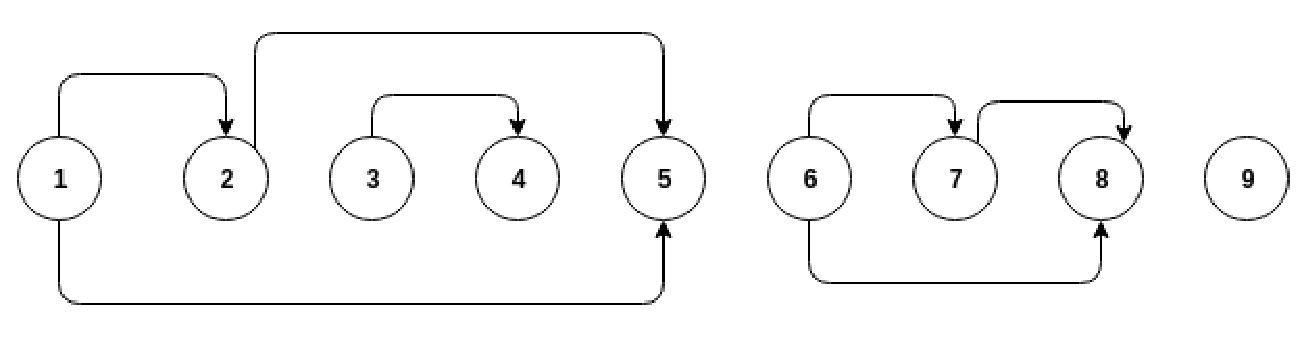
\includegraphics[width=0.7\textwidth]{digraph1.eps}
    %\resizebox{100mm}{!} {\includegraphics *{digraph1.png}}
    %\resizebox{50mm}{!} {\includegraphics *{iitm.eps}}
    \caption {Digraph for the above example.}
  %\label{fig:iitm}
  \end{center}
\end{figure}
\\
\noindent
\textbf{Largest Non-crossing set: $C(S)$}\\
2 edges $(u,v)$ and $(w,z)$ are said to cross each other if $u\leq w < v \leq z$ or $w\leq u < z \leq v$. An edge set E' is said to be non-crossing if no 2 edges in the set cross each other. The size of the maximal non-crossing edge set is denoted as $C(S).$ $C(S)$ for the example is 5, the red edges shown below.
\begin{figure}[htpb]
  \begin{center}
  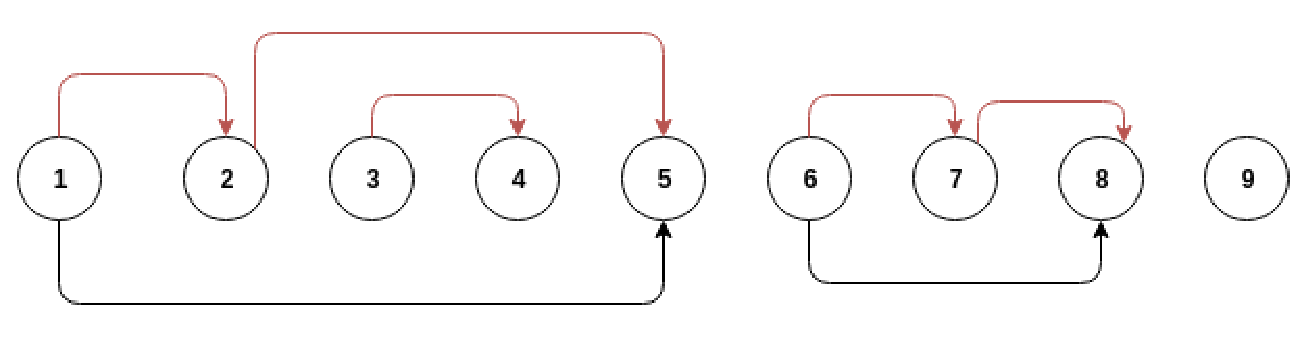
\includegraphics[width=0.7\textwidth]{digraph2.eps}
    %\resizebox{100mm}{!} {\includegraphics *{digraph2.png}}
    %\resizebox{50mm}{!} {\includegraphics *{iitm.eps}}
    \caption {The highlighted red edges belong to the maximum non-crosssing edge set}
  %\label{fig:iitm}
  \end{center}
\end{figure}
\\
\noindent
There is a \textbf{Polynomial time algorithm using Dynamic Programming to find the $C(S)$}. Let $DP(i,j)$ represent the maximum non-crossing set for the sub-graph with the vertices $[i,j]$. \\
\textbf{Base case:}
\begin{enumerate}
    \item $DP(i,i)$ = 0 $\forall i$.
    \item $DP(i,i+1)$ = 1 if $(i,i+1) \in$ E
    \item $DP(i,i+1)$ = 0 if $(i,i+1) \notin$ E
\end{enumerate}
\[ DP(i,j) = \begin{cases} 
      max(DP(i,j),DP(i,l) + DP(l,j)) & \forall l \in [i+1,j-1] \\
      max(DP(i,j),DP(i+1,j-1) + 1) & (i,j) \in E \\
      max(DP(i,j),DP(i+1,j-1)) & (i,j) \notin E \\
   \end{cases}
\]
The explanation for the construction of $DP(i,j)$ using the above procedure is as follows:
\begin{enumerate}
    \item $max(DP(i,j),DP(i,l) + DP(l,j))$  $\forall$ $l$ $\in$ $[i+1,j-1]$ deals with all the cases where the non-crossing edge sets are possible without using edge $(i,j)$.
    \item $max(DP(i,j),DP(i+1,j-1) + x) (i,j) \in E$ deals with the cases where edge $(i,j)$ is present. $x$ is 0 or 1 depending on whether $(i,j) \in$ E. 
\end{enumerate}
\noindent
\textbf{Obtaining optimal moves for 1-Block Merging}\\
Obtaining optimal set of moves starts by finding $bm(\pi)$. Which follows as a result of following lemmas.\\
\textbf{Lemma 2.1:}\\
Any valid block move from $S$ which results in $S'$ follows that $C(S')$ $\leq$ $C(S)$ + 1\\
\textbf{Proof:}\\
If the block moved is $[i,j]$, then from the source side(Sequence from which the block is moved) there will be a loss of 1 or 0 to $C(S)$ and the destination side( Where the block is moved to) will add at most 1 to $C(S)$. Let $NC(S)$ denote the non-crossing edge set for $S$.
\begin{enumerate}
    \item Let the source side for block $[i,j]$ looks like $a,i,...,j,b.$ If $(a,i)$ $\in$ $NC(S)$ and $(j,b)$ $\in$ $NC(S)$, then $(a,b)$ $\in NC(S')$ which make a total loss of 1 in source side. If any one of the edge is absent, then $(a,b)$ $\notin$ $NC(S')$ which also incurs a loss of 1. If both the edges $(a,i)$ and $(j,b)$ are absent, then the loss is 0.
    \item In the destination side let the block be inserted between $c,d$. Then new edges added will be $(c,i)$ and $(j,d)$ is $(c,d)$ is present, which adds 1 to $C(S)$. If one of the $c$ or $d$ is absent, only one edge will be added. So in the destination side there is a profit of maximum 1.
\end{enumerate}
A maximum profit of 1 on destination side and maximum loss of 1 on source side gets us to the result that $C(S') \leq  C(S) + 1.$\\~\\
\textbf{Lemma 2.2:}\\
Given any sequence set $S$, there exist a block move which will result in $S'$ such that $C(S')$ = $C(S)$ + 1\\
\textbf{Proof:}\\
A block is said be free if there is no edge of the form $(i,j)$ such that only one of $i$ or $j$ belong to the block and the other does not. As we can see movement of a free block will induce 0 loss in source side and a profit of 1 in destination side, hence increase in $C(S)$ by 1. So it is left to prove that \textbf{we can find a free block in any $S$ if it is not $id_n$}.
\begin{enumerate}
    \item If all the edges are unit edges of the form $(i,i+1)$ and still we have not reached $id_n$, then all the blocks are free blocks.
    \item If there exist a non-unit edge, find a non-unit edge such that it doesn't contain any non-unit edge in it. Let that edge be $(i,j)$. Since $(i,j) \in NC(S)$, $(i,i+1) \notin$ $NC(S)$ and $(j-1,j) \notin NC(S)$. As $i+1,...j-1$ contains only unit edge, blocks from $i+1,...j-1$ is a free block.
\end{enumerate}
Hence there exists a move for every $S$ (which is not $id_n$) to $S'$ such that $C(S')$ = $C(S)$ + 1.\\~\\

\noindent
\textbf{Lemma 2.3:} \\
$bm(\pi) = n - 1 - C(S)$.\\
\textbf{Proof:}\\
We prove this by showing $bm(\pi)$ $\leq$ $n - 1 - C(S)$ and $bm(\pi)$ $\geq$ $n - 1 - C(S)$.\\
$bm(\pi)$ $\geq$ $n - 1 - C(S)$:\\ Because of the Lemma 2.1 every block move can only increase $C(S)$ by 1. In the optimal set of moves we start with $C(S)$ and we complete with n-1. Let $S_1 ,S_2,.. S_{bm(\pi)}$ be the sets obtained after each move in the optimal set of moves. $C(S_i) \leq C(S_{i-1}) + 1$, Hence $C(S_{bm(\pi)}$ $\leq$ C($S$) + $bm(\pi)$. Since $C(S_{bm(\pi)}$ = $n-1$, $C(S)$ $\geq$ $n-1-C(S).$\\
$bm(\pi)$ $\leq$ $n - 1 - C(S)$:\\ The proof of this is by Induction on $r = n-1-C(S).$ For $r = 0$, we take $id_n$, so $bm(\pi)$ = 0. Therefore $bm(\pi) \leq  n - 1 - C(S)$. So lets assume that for $r = y$, $bm(\pi) \leq  n-1-C(S)$. Now lets take a case of $C(S)$ such that $r = y+1$. We know from Lemma 2.2 that there exist a block move which can result in $C(S)+1$. So we make that move hence obtaining $\pi'$. Now $\pi'$ has $r = y,$ so $bm(\pi') \leq n-1-(C(S)+1)$. Which is equivalent to $bm(\pi') + 1 \leq  n-1-C(S)$. $bm(\pi)$ is the minimum number of moves to sort $\pi$. So $bm(\pi) \leq$ $bm(\pi') + 1 \leq  n-1-C(S)$. So for $r = y+1$, $bm(\pi) \leq n-1-C(S)$. By induction hypothesis $bm(\pi)$ $\leq n - 1 - C(S)$ for all $r$.\\
As the inequalities are in proved in both the directions, $bm(\pi) = n-1-C(S)$.\\
\noindent
Now as we know that $bm(\pi) = n-1-C(S)$ and how to find a move which results in increase in $C(S)$, we can obtain $id_n$ in $n-1-C(S)$ such moves which can be done in $O(n^4)$ time complexity. Now that we have an exact solution for 1-block merging it will serve as 2 approximation to block sorting.

\begin{algorithm}
\caption{Optimal Block Merging}\label{euclid}
\begin{algorithmic}[1]
\Procedure{Block Merge($\pi$,$C$)}{}
\State \textbf{Input: } $\pi \text{ is a permutation and }\textit{C} \text{ is a maximum non-crossing edge set for } \pi$ 
\While{$\pi$ $\neq$ id$_n$} 
\State $\textit{B} \gets \text{Free block with respect to }\textit{C}$ 
\State $\text{Let } u,v \text{ be the first and last element of the block respectively}$
\If {$\textit{B}$ has a predecessor } 
\State $\text{Merge } \textit{B} \text{ with its predecessor}$
\If{$(u-1,l)$}
\State $C = C\backslash(u-1,l)\text{ and } C = C\cup(v,l)$
\EndIf
\State $C = C\cup(u-1,u)$
\Else
\State $\text{Merge } \textit{B} \text{ with its successor}$
\If{$(l,v+1)$}
\State $C = C\backslash(l,v+1)\text{ and } C = C\cup(l,u)$
\EndIf
\State $C = C\cup(v,v+1)$
\EndIf
\EndWhile
\EndProcedure
\end{algorithmic}
\end{algorithm}


%%%%%%%%%%%%%%%%%%%%%%%%%%%%%%%%%%%%%%%%%%%%%%%%%%%%%%%%%%%%
% Appendices.

\appendix

\chapter{A SAMPLE APPENDIX}

Just put in text as you would into any chapter with sections and
whatnot.  Thats the end of it.

%%%%%%%%%%%%%%%%%%%%%%%%%%%%%%%%%%%%%%%%%%%%%%%%%%%%%%%%%%%%
% Bibliography.

\begin{singlespace}
  \bibliography{refs}
\end{singlespace}


%%%%%%%%%%%%%%%%%%%%%%%%%%%%%%%%%%%%%%%%%%%%%%%%%%%%%%%%%%%%
% List of papers

\listofpapers

\begin{enumerate}  
\item Authors....  \newblock
 Title...
  \newblock {\em Journal}, Volume,
  Page, (year).
\end{enumerate}  

\end{document}
